\chapter{Effects of Patient-Specific Variability in Inconsistent End-Expiratory Diaphragm Position On the Quantification of Left Ventricular Cardiac Strains}

\textit{Adapted from...}

\section{Synopsis}
	\noindent \textbf{Purpose:}  To determine if normal inconsistency in end-expiratory diaphragm position between separate image acquisitions significantly affects estimates of cardiac strains.

	\noindent \textbf{Materials and Methods:} We enrolled 17 subjects, including seven patients with heart disease. For each subject, we measured the range of end-expiratory positions during 10 separate breath-holds. The imaging protocol comprised two ventricular long-axis and three short-axis slices of navigator-gated 2D cine displacement encoding with stimulated echoes (DENSE) cardiac magnetic resonance (MR). To simulate end-expiratory position inconsistency, DENSE images were each acquired at the patient-specific minimum, middle, and maximum end-expiratory positions; a repeated acquisition at the middle position was used to quantify variability independent of end-expiratory differences. Differences and variability of left ventricular peak strains were compared using analysis of variance and Student’s t-test.
	
	\noindent \textbf{Results:} The range of end-expiratory positions across 10~breath-holds was 10~$\pm$~4~mm. There were no significant differences in global or regional peak radial, circumferential, or longitudinal strains measured at the different end-expiratory positions (p~=~0.17–--0.98). In general, there were also no differences in variability in global or regional peak strains between inconsistent (minimum, middle, and maximum) and consistent (two acquisitions from middle position) end-expiratory positions (p~=~0.10--–0.95). With at least 80\% power, the study had an ability to detect global differences of 4.7\%, 1.0\%, and 1.7\% (absolute) between end-expiratory positions for radial, circumferential, and longitudinal strains, respectively.
	
	\noindent \textbf{Conclusion:} Measurements of left ventricular peak strains with DENSE cardiac MR are relatively insensitive to normal changes in end-expiratory position between separate image acquisitions.
	
	\noindent \textbf{Keywords:} Cardiac Strains, Breath-holds, DENSE, Respiratory Navigator Gating
	
\newpage

\section{Background}
	Cardiac strains describe the deformation of myocardial tissue during contraction and relaxation. Measures of cardiac strains have been shown to be superior predictors of outcomes, such as mortality, compared to traditional measures of cardiac function or traditional clinical risk factors alone \cite{Stanton2009}. Imaging can non-invasively assess cardiac strains using echocardiographic techniques such as speckle tracking \cite{Amundsen2006} and cardiovascular magnetic resonance (MR) techniques such as myocardial feature tracking \cite{Hor2010}, myocardial tissue tagging \cite{Axel1989,Zerhouni1988}, phase velocity mapping \cite{Pelc1994}, strain encoding \cite{Osman2001}, and displacement encoding with stimulated echoes (DENSE) \cite{Aletras1999b,Aletras1999c}.

	Peak strains vary longitudinally throughout the left ventricle \cite{Kuijer2002,Moore2000,Young1994a,Feng2009,NasiraeiMoghaddam2010,Donekal2013a,Suever2017}. For example, previous studies have shown that left ventricular radial, circumferential, and longitudinal strains vary between the base and apex by up to 14\%, 5\%, and 5\% (absolute), respectively \cite{Kuijer2002,Moore2000,Young1994a,Feng2009,NasiraeiMoghaddam2010,Donekal2013a,Suever2017}. Cardiac MR images are often acquired during end-expiratory breath-holds to minimize respiratory motion artifacts. However, it is often difficult to achieve consistency in end-expiratory diaphragm position between successive breath holds, and variations of 4 to 13 mm are normal [17–21] \cite{Liu1993,Wang1995a,Taylor1997a,Holland1998c,Fischer2006a}. Inconsistent end-expiratory positions will impact the position of the heart with respect to the imaging plane (Figure~\ref{fig:diaphragmTranslation}). For example, previous studies have reported short-axis and long-axis through-plane displacements of up to 14 mm due to displacement of diaphragm position between breath-holds \cite{Slomka2007,Swingen2003}, and other studies have reported that the superior/inferior position of the heart can displace 55-92\% of the displacement of the diaphragm position \cite{Wang1995b,McLeish2002}. Because peak strains vary throughout the left ventricle, we hypothesize that translation of the heart with respect to the imaging plane to result in differences and variability in measured strains.

	To our knowledge, no study has evaluated the sensitivity of cardiac strains to natural end-expiratory position variability. This is an important knowledge gap, especially since the use of cardiac strains is increasing dramatically both in research and clinical practice. The purpose of this study was to determine if normal inconsistency in end-expiratory position significantly affects the quantification of cardiac strains and therefore results in higher variability in measured cardiac strains compared to strains measured at a consistent end-expiratory position.
	
	\begin{figure} 
		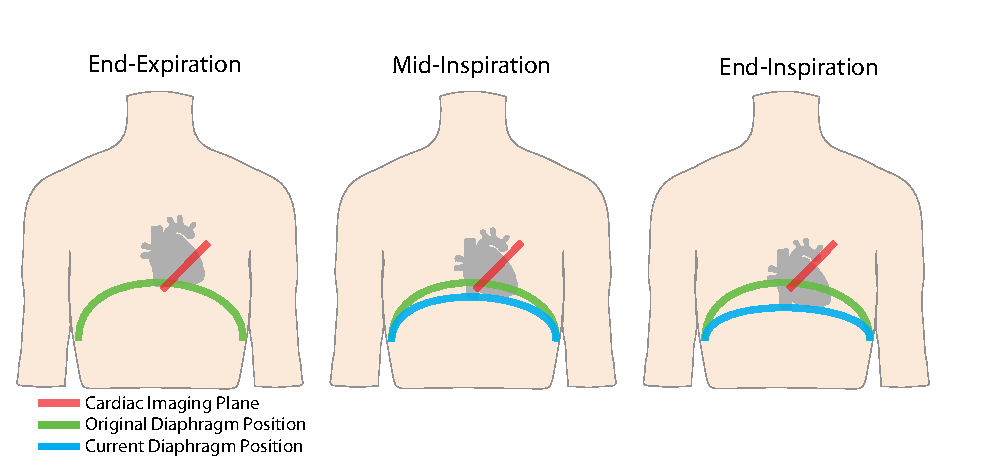
\includegraphics{figures/strainpaper/Fig1-range_of_diaphragm_position_breathing}
		\caption[During respiration, diaphragm motion causes the heart to translate a significant distance while the imaging plane remains fixed]{\textbf{During respiration, diaphragm motion causes the heart to translate a significant distance while the imaging plane remains fixed.}}
		\label{fig:diaphragmTranslation}
	\end{figure}

\section{Methods}

\subsection{Subjects}
	The study protocol was approved by the local Institutional Review Board. Ten healthy volunteers with no known cardiovascular disease or chronic illnesses and 7 patients with a history of heart disease (known diagnosis of heart failure, cardiomyopathy, or myocardial infarction) provided written informed consent. Image acquisitions were performed on a 3T Siemens Tim Trio (Siemens Healthcare, Erlangen, Germany) scanner with a 6-element chest coil and a 24-element spine coil.

\subsection{Quantification of Inconsistent End-Expiratory Positions}
	To determine the inconsistency in end-expiratory positions for each subject, a respiratory navigator sequence measured the diaphragm position (Figure~\ref{fig:navGatingExplanationCartoon}) during 10 consecutive breath-holds. During each breath-hold, the diaphragm position was imaged three times per second over a period of 10 seconds for 30 total measurements. No cardiac image data were collected during these acquisitions. The mode of the 30 diaphragm positions defined the measured end-expiratory position of that breath-hold. The patient-specific minimum, middle, and maximum end-expiratory positions were defined from the series of 10 breath-holds (Figure~\ref{fig:translatedAccWindowBlue}).
	
	\begin{figure} 
		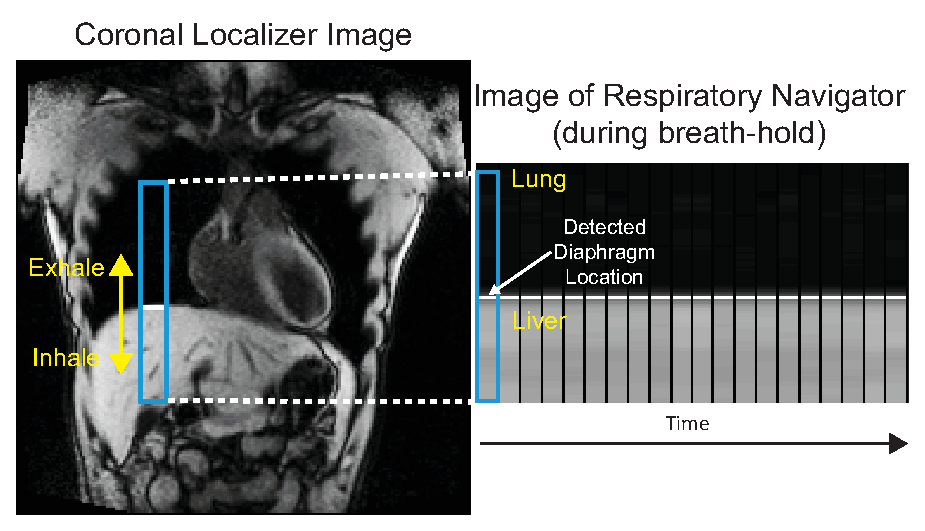
\includegraphics{figures/strainpaper/Fig2-navigator_gating_explanation_NoAccWin}
		\caption[Respiratory navigator gating]{\textbf{Respiratory navigator gating.} (Left) The diaphragm position was measured at the high-contrast interface between the lung (dark) and the liver (bright). (Right) Image of a measured diaphragm position over time during a breath-hold.}
		\label{fig:navGatingExplanationCartoon}
	\end{figure}
	
	\begin{figure} 
		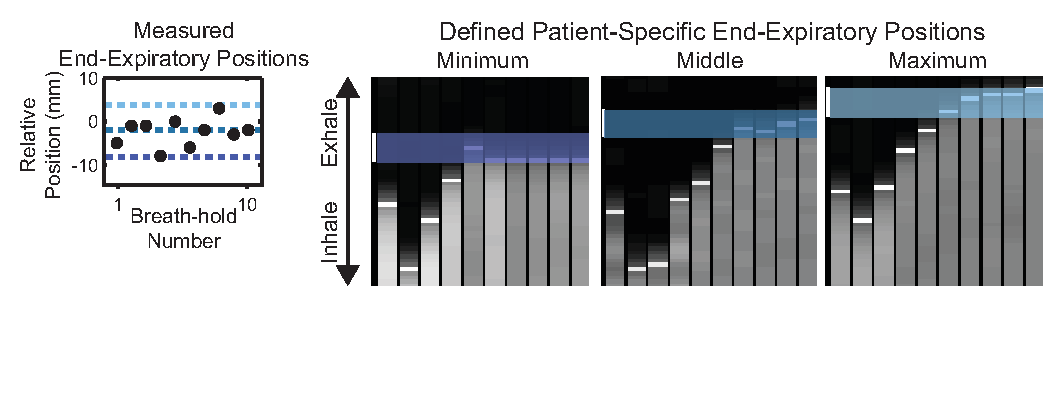
\includegraphics{figures/strainpaper/Fig3-definedTranslatedAccWindow}
		\caption[A respiratory navigator was used to measure end-expiratory positions to define the patient-specific minimum, middle, and maximum end-expiratory positions]{\textbf{A respiratory navigator was used to measure end-expiratory positions to define the patient-specific minimum, middle, and maximum end-expiratory positions.} The minimum position was defined as being closer to the end-inspiratory position while the maximum position was defined as being closer to the end-expiratory position.}
		\label{fig:translatedAccWindowBlue}
	\end{figure}
	
	DENSE Acquisition
	For each subject, navigator-gated 2D spiral cine DENSE in 2-chamber and 4-chamber long-axis and basal, mid-ventricular, and apical short-axis orientations of the left ventricle were acquired four times. Specifically, all image orientations were acquired with the navigator acceptance window prescribed at the patient-specific maximum and minimum end-expiratory positions, and twice in the middle position to quantify variability in strain independent of end-expiratory position variability (Figure 3). A navigator feedback system, which used an angled mirror and projector screen placed at the back of the scanner bore, was used to facilitate quicker acquisitions by enabling subjects to view the navigator acceptance window position in real-time during image acquisition [26]. For each end-expiratory position, all image orientations were acquired within a single navigator-gated scan.
	Prospective ECG gating was used during DENSE acquisitions. The number of cardiac phases ranged from 31 to 49 and varied based on subject heart rate. Additional DENSE imaging parameters included: spiral interleaves = 6, FOV = 360x360 mm2, pixel spacing = 2.8x2.8 mm2, slice thickness = 8 mm, TE = 1.1 ms, TR = 17 ms, variable flip angle = 20°, displacement encoding = 0.06 cyc/mm [27], through-plane dephasing = 0.08 cyc/mm [28], CSPAMM echo suppression [29], and view sharing. A dual-navigator strategy was used, requiring the diaphragm to be within the navigator acceptance window (±3 mm) both before and after the data acquisition during each R-R interval [30].
	DENSE Post-Processing
	DENSE image data were analyzed using the open-source software, DENSEanalysis [31]. For each image orientation, the left ventricular myocardium was manually delineated using epicardial and endocardial contours and an end-diastolic and end-systolic cardiac phase [32]. Post-processing and segmentation were performed as described by Suever et al. [32]. Seed points indicating unwrapped phase data were manually selected, and a path-following algorithm was used to unwrap the displacement-encoded phase data. The resulting displacement trajectories were further processed by applying spatial smoothing and temporal fitting as previously described [33].
	Two-dimensional Lagrangian strains were computed from the smoothed trajectories over the entire cardiac cycle. Radial and circumferential strains were computed from the short-axis images and longitudinal strain was computed from the long-axis images. Global peak strains were calculated by averaging the mean strain curves of all the myocardial segments and identifying the peak of the global mean curve. Regional peak strains were computed by averaging the strain curves from all the myocardial segments for a given region and identifying the peak of the regional curve. Segmental peak strains were computed by identifying the peak of the strain curve for each myocardial segment. For peak longitudinal strain computation, pixels within 10% of left ventricular longitudinal length from the most basal and apical regions were excluded because of the increased noise which is typically observed in the strain curves in those regions. Peak strain was defined as positive for thickening (radial) and negative for shortening (circumferential and longitudinal).
	Statistics
	Statistical analyses were performed using R version 3.2.2 (R Foundation for Statistical Computing, Vienna, Austria). All continuous variables were expressed as mean ± standard deviation or range. Cardiac strains were tested for normality using a Shapiro-Wilk test.
	To quantify mean differences in cardiac strains due to inconsistent end-expiratory positions (minimum, middle, and maximum positions), cardiac strains were compared between the patient-specific acceptance window positions using a two-way analysis of variance (ANOVA) with repeated measures with group (healthy vs patient) and acceptance window position as the independent factors. A Scheirer-Ray-Hare test was used for data determined to be non-normally distributed [34]. Using the results of the two-way ANOVA or Scheirer-Ray-Hare test, the interaction between group and acceptance window position on cardiac strains was determined. If there was no interaction between group and acceptance window position, the groups were combined and mean differences due to inconsistent end-expiratory positions were quantified by comparing cardiac strains between acceptance window positions using a one-way ANOVA with repeated measures with acceptance window position as the independent factor. A Friedman test was used for data determined to be non-normally distributed [34].
	To quantify variability due to inconsistent end-expiratory positions, the standard deviations of strains were compared between the inconsistent positions (maximum, middle, and minimum) and consistent positions (two acquisitions at the middle position) using a Student’s t-test. For all statistical tests, significance was defined as p < 0.05. Bland-Altman analysis [35] was used to assess the reproducibility of each measurement using inter-test 95% limits of agreement defined using the two measurements from the middle position. Inconsistency in end-expiratory position across ten separate breath-holds for each subject was reported using both ranges and standard deviations from the ten breath-holds, and these values were compared between patients and healthy controls.
	Power analyses were performed to quantify the ability of this study to detect meaningful differences in strain between the different end-expiratory positions. Because repeated-measures ANOVAs were used to detect differences, and because equations for power are not readily available for repeated-measures ANOVA, simulations were performed to estimate power. Specifically, for each strain, 10,000 iterations were performed. For each iteration, strain values for the minimum end-expiratory position were randomly drawn from a normal distribution using the mean and standard deviation across the subjects measured in this study.  The number of strain values drawn corresponded with the number of subjects (healthy and patients combined). For a given difference to detect, δ, values at the two other end-expiratory positions were calculated by adding δ/2 and δ to the values at the minimum position. Measurement variability was then added to those two end-expiratory positions by drawing random values from a normal distribution with zero mean and a standard deviation equal to the measured average standard deviation of the differences between any two positions. In this manner, each iteration simulated a mean difference of δ between the minimum and maximum breath-hold positions and included typical inter-test measurement variability. The percentage of iterations for which a repeated-measures ANOVA yielded a significant result (p < 0.05) was the estimate of power. The 95% confidence interval of that estimate was calculated from the normal approximation to the binomial distribution with N = 10,000. The values of δ that yielded at least 80% power were reported separately for global and regional strains.
	
	

